\documentclass[journal]{IEEEtran}

\usepackage{cite}
\usepackage[T1]{fontenc}
\usepackage{newtxtext,newtxmath}
\usepackage{amsmath}
\usepackage{graphicx}
\usepackage{booktabs}
\usepackage{array}
\usepackage{xurl}
\usepackage[hidelinks]{hyperref}

\graphicspath{{figures/}}
\hyphenation{Edge-Mango Xiao-mi Albu-men-ta-tions}

\begin{document}

\title{Edge-Mango: Mobile Inference of Mechanical Damage through Multimodal Feature Distillation}

\author{%
\begin{tabular}[t]{c}
Gabriel Ysidro\\
Universidad de Lima\\
Lima, Peru\\
20222848@aloe.ulima.edu.pe
\end{tabular}
\hspace{3em}
\begin{tabular}[t]{c}
Lourdes Ram\'irez\\
Universidad de Lima\\
Lima, Peru\\
lramirez@ulima.edu.pe
\end{tabular}}

\maketitle

\begin{abstract}
Impact-induced mechanical damage is one of the main causes of rejection in export mangoes, and during its first hours it remains latent beneath the skin, where visual inspection and RGB cameras cannot detect it. This work evaluates whether an 850 nm NIR camera provides information about latent damage and whether that information can be transferred, through cross-modal knowledge distillation (CrossKD), to a lightweight segmentation model that receives only RGB images at inference. A dataset of 3966 aligned RGB-NIR pairs from 125 Edwards mangoes was built, photographed before a controlled impact and every two hours over the following 12 hours, with the damage annotated as polygons. Using a YOLOv8n-seg architecture with about 3.4 million parameters, five configurations that differ only in their input or teacher were trained and evaluated with lot-wise cross-validation. Adding NIR to the input raised the latent-damage AP50 from 0.306 to 0.388, with improvements in all five lots and a probability of practical improvement of 0.953, above the 0.95 threshold. The RGB student distilled from the RGB + NIR teacher reached 0.354, against 0.318 with an RGB teacher, an inconclusive difference (probability 0.689). On the NPU of a Xiaomi 14T, the student took 17.6 ms per image and the full system, with a preceding mango detector, ran offline at 1.25 frames per second with 519 MB of memory, although at a real environment test it flagged damage on every fruit. With a single seed, the results support that NIR carries information about latent damage, but not that distillation carries it over to RGB.
\end{abstract}

\begin{IEEEkeywords}
Mechanical damage, agricultural export, multimodal features, knowledge distillation, mobile inference
\end{IEEEkeywords}

\section{Introduction}\label{sec:intro}
Agro-exports account for most of Peru's non-traditional shipments~\cite{soriano2025}, and mango (\emph{Mangifera indica} L.) places the country among the main suppliers to markets that demand high quality, such as the European Union and the United States~\cite{cosio2026}. Maintaining that position requires a supply chain that preserves the physical integrity of the fruit from packing to the final consumer~\cite{jayathilaka2026}, a necessary condition for accessing high-value markets~\cite{sanchez2023}. However, mechanical damage from drops or impacts is the main cause of commercial rejection in postharvest~\cite{le2022}.

Mechanical damage, which appears as bruises caused by compression, impact or vibration during harvest, packing and transport, is one of the main factors of value loss in the fruit industry~\cite{liu2025}. A bruise on a fruit of ten cubic centimeters can reduce its shelf life by up to 50\% along the logistics chain~\cite{gamez2022}, because the blow raises the respiration rate and triggers enzymatic browning catalyzed by polyphenol oxidase~\cite{queiroz2008}, reactions that are not mitigated even with active packaging~\cite{hao2025}. During its first hours, the lesion remains optically latent beneath the skin and passes conventional quality controls.

The Codex standard for mango requires fruit of all categories to be free of marked bruises and admits only healed bruises of 3 to 7~cm$^2$, depending on the category and size~\cite{codex2005}. In Peru, NTP 011.010:2020 covers the Edwards variety~\cite{inacal2020}, and the technical datasheet for Premium-category Edwards mango requires fruit free of bruises~\cite{ficha2021}. A lesion that is still latent during inspection cannot be measured against these limits and may become apparent after the fruit has already been graded and packed.

On the other hand, inspection in packing plants relies on subjective manual sampling, and vision systems based on RGB images only identify deterioration once browning has emerged at the surface. In contrast, hyperspectral imaging allows non-destructive estimation of internal properties of the fruit; for example, Zhang \emph{et al.}~\cite{zhang2022} predicted mechanical parameters of apples from their spectral response using support vector machines, which shows that the spectrum records tissue information that is not visible at the surface. However, these solutions assume costly sensors and high-performance servers at inference time, conditions that hinder their adoption in Peruvian packing lines.

The contribution of this research is a system for early detection of latent mechanical damage in mangoes adapted to those conditions. Through cross-modal knowledge distillation, a lightweight segmentation model learns, during training, from a teacher that receives RGB and near-infrared (NIR) images, and at inference it operates only on RGB images from commercial cameras. The solution covers the construction of a paired multimodal dataset under a standardized impact protocol, the training of the teacher and the student, and the offline deployment of the student on a phone with Kotlin and LiteRT, where its latency, memory and size are measured on CPU, GPU and NPU.

Section~\ref{sec:related} reviews related work; Section~\ref{sec:theory}, the theoretical framework; Section~\ref{sec:method}, the methodology; Section~\ref{sec:exp}, the experimentation; Section~\ref{sec:results}, the results; Section~\ref{sec:discussion}, the discussion; and Sections~\ref{sec:conclusions} and~\ref{sec:future}, the conclusions and future work.

\section{Related Work}\label{sec:related}
The non-destructive assessment of mechanical damage in fruit moved from destructive chemical analysis to optical spectroscopy and, more recently, to deep learning. However, the literature shows a persistent dichotomy: accurate systems depend on inaccessible hardware, while accessible systems lack the accuracy needed for latent defects.

Internal mechanical damage is imperceptible in the visible spectrum during the early stages, which consolidated the use of spectral and NIR imaging. V\'elez Rivera \emph{et al.}~\cite{velez2014} detected early damage in mango with 650 to 1100 nm hyperspectral images and a k-NN classifier, with 97.9\% of pixels correctly classified on the third day, although on manually selected regions and with a random pixel split of the same fruits. Yao \emph{et al.}~\cite{yao2024} estimated the time elapsed since a mild bruise in mango by combining hyperspectral spectral and texture features with a convolutional network. Okere \emph{et al.}~\cite{okere2023} detected early bruises in pomegranate with hyperspectral images and a simple two-layer neural network. Castillo-Girones \emph{et al.}~\cite{castillo2024} detected subsurface bruises in plum with 430 to 1000 nm spectral images and convolutional networks such as HSCNN, using only three wavelengths. Gulzar and \"Unal~\cite{gulzar2025} proposed PlmNet, a convolutional network to detect plum bruises according to the time elapsed since the blow, using NIR images. Li \emph{et al.}~\cite{li2023} discriminated the time elapsed since a light bruise in yellow peaches (2, 8, 24 and 48~h) by combining spectral and texture features with Random Forest, with 98.33\% accuracy. Pourdarbani \emph{et al.}~\cite{pourdarbani2023} classified lemon bruises at 8 and 16 hours after the blow with 3D-CNN networks on 400 to 1100 nm hyperspectral cubes, with 90.47\% accuracy with ResNet. Yuan \emph{et al.}~\cite{yuan2022} showed that a broadband NIR camera (900 to 2350 nm) with a convolutional network suffices to detect apple bruises in their first half hour, without the full hyperspectral cube. Yan \emph{et al.}~\cite{yan2025} combined a NIR camera with MCC-DeepLabV3+, a lightweight segmenter built on MobileNetV2, to delimit pear bruises of less than 30 minutes that cannot be distinguished with the naked eye. The problem common to these works is that they assume costly spectral or NIR cameras at inference.

To improve robustness, other works fused several sensors. He \emph{et al.}~\cite{he2025} combined thermal images with flexible spectral sensing to classify mangoes with cold damage and bruises, with up to 95.24\% accuracy. Y. Wang \emph{et al.}~\cite{wang2025} proposed MECN-net, which integrates RGB images, thermal images and dielectric properties measured with flexible sensors, with 95.5\% accuracy on the same task. These solutions improve accuracy in controlled environments, but integrating and synchronizing several cameras, and even contact sensors, makes them unviable for most packing plants in Peru.

Cross-modal knowledge distillation (CMKD) seeks to close the gap between the accuracy of costly hardware and the accessibility of RGB sensors. Xiong \emph{et al.}~\cite{xiong2023} generalized the multimodal-teacher, unimodal-student scheme to segment gliomas in magnetic resonance imaging, combining the imitation of the teacher's softened outputs with that of regional features from several of its layers. Chen \emph{et al.}~\cite{chen2022} formalized this principle as learning with privileged information, with a pixel-level distillation regularized to attenuate the teacher's errors and an image-level contrastive one. Huo \emph{et al.}~\cite{huo2024} identified the gap between modalities, that is, the modal imbalance and the misalignment of soft labels, as the cause of the low performance of conventional distillation, and proposed C2KD, which mitigates it with bidirectional distillation and the selection of aligned samples. J. Wang \emph{et al.}~\cite{wang2024} proposed CrossKD, which instead of imitating feature maps makes the student's intermediate features pass through the teacher's head and compares those cross predictions with the teacher's, and raised the AP of a GFL detector with ResNet-50 on COCO from 40.2 to 43.7. Z. Feng \emph{et al.}~\cite{feng2023} proposed CEKD, in which an RGB-thermal fusion teacher enriched with edge information guides a student that segments scenes using only thermal images. Yoon \emph{et al.}~\cite{yoon2026} improved a detector that operates only on thermal images by distilling knowledge from the visible modality into it. However, none of these works reports the export of their students to an edge device.

Finally, distilled models must run on resource-limited hardware. Fatehi \emph{et al.}~\cite{fatehi2025} distilled a YOLOv9c detector into a YOLOv9t student to detect roses in the field and improved both its accuracy and its speed. The work closest to this proposal is that of Poojitha \emph{et al.}~\cite{poojitha2026}, who distilled an RGB-thermal teacher into a student that operates only on RGB at inference, with 75\% mAP against the teacher's 80\% (94\% recovered) and ten times fewer parameters. Unlike the previous works, that work reports the cost of edge inference, with 28 FPS and 0.051 J per inference on an NVIDIA Jetson AGX Orin, although on driving scenes and not on latent organic defects.

Consequently, the gap that this research seeks to close is the lack of a system that decouples the detection of latent defects from costly spectral equipment. An asymmetric architecture is proposed in which the NIR sensor intervenes only during training, through a teacher that receives RGB and NIR images, while the student, a YOLOv8n-seg segmenter, learns from that teacher to recognize the damage in RGB images and runs offline on a phone.

\section{Theoretical Framework}\label{sec:theory}
This section presents the foundations of the proposal: the physiology of mechanical damage, the information provided by each modality, cross-modal knowledge distillation, edge inference and the evaluation metrics.

\subsection{Mechanical Damage (Detection Target)}\label{sec:damage}
In postharvest physiology, mechanical damage is the physical disruption of the cellular and tissue integrity of the fruit by compression, impact or vibration forces. That energy ruptures the vacuolar membranes and mixes the enzyme polyphenol oxidase with phenolic substrates, which catalyzes internal enzymatic browning~\cite{queiroz2008}.

The challenge for computer vision is that the initial damage occurs in the underlying pulp and takes time to manifest in the epidermis, which makes it imperceptible to the human eye and to RGB sensors during packing (Fig.~\ref{fig:damage}).

\begin{figure}[!t]
\centering
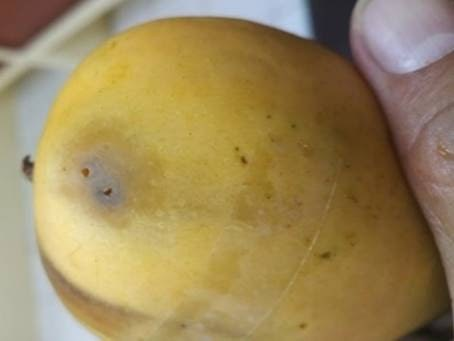
\includegraphics[width=0.8\columnwidth]{fig1_damage.jpg}
\caption{Mechanical damage in mangoes. Note. Extracted from ``Survey of phytosanitary problems at harvest and postharvest of mango (\emph{Mangifera indica} L.) in the Yaut\'an Valley, Casma Province, Ancash''~\cite{palomo2023}.}
\label{fig:damage}
\end{figure}

\subsection{Multimodal Features in Computer Vision}\label{sec:multimodal}
This work employs two optical channels. The visible spectrum (RGB, 400 to 700 nm) records the geometry, color and texture of the skin, but penetrates little into the tissue. In the near infrared at 850 nm, light interacts with the O-H bonds of water and the C-H bonds of carbohydrates in the internal tissue; when the membranes rupture, the redistribution of fluids and the changes in light scattering alter the reflectance, so that the internal damage becomes measurable intensity variations before surface oxidation.

\subsection{Cross-Modal Knowledge Distillation}\label{sec:crossmodal}
Cross-modal knowledge distillation allows a student model to learn useful representations in an impoverished modality (RGB) guided by a teacher that, during training, had access to a richer modality~\cite{gupta2016}. In the present work, the teacher receives RGB and NIR images, while the student receives only RGB.

Instead of training the student solely with the manual labels of the defect, the knowledge of the teacher is also exploited~\cite{gou2021}. A classic alternative is to imitate intermediate features with a squared error, as in FitNets~\cite{romero2015}, which forces the student to reproduce features of the teacher even if they are not in its input. CrossKD~\cite{wang2024}, in turn, moves the imitation to the predictions: the intermediate features of the student's head pass through the remaining layers of the frozen teacher's head, and the resulting cross prediction is brought closer to the teacher's own prediction. The loss function adds the student's detection error against the labels, $\mathcal{L}_{\mathrm{Task}}$, and the classification, $\mathcal{L}_{\mathrm{KD,cls}}$, and box, $\mathcal{L}_{\mathrm{KD,reg}}$, distillation terms.
\begin{equation}\label{eq:loss}
\mathcal{L}_{\mathrm{Total}} = \mathcal{L}_{\mathrm{Task}} + \lambda_{\mathrm{cls}}\,\mathcal{L}_{\mathrm{KD,cls}} + \lambda_{\mathrm{reg}}\,\mathcal{L}_{\mathrm{KD,reg}}
\end{equation}
In the equation, $\lambda_{\mathrm{cls}}$ and $\lambda_{\mathrm{reg}}$ weight each distillation term (both equal 1.0 in this work). The classification term is the Quality Focal Loss (with $\beta = 1$) between the cross classification and the teacher's, equivalent to a Bernoulli Kullback-Leibler divergence; the box term is the GIoU between the cross box and the teacher's, weighted by the maximum class probability that the teacher assigns to each cell. Thus, the student is penalized only for the differences that change the detection decision of a teacher that remains frozen, and not for failing to reproduce features specific to the NIR.

\subsection{Edge Computing and Efficient Inference}\label{sec:edge}
Edge computing moves inference from centralized servers to devices close to the data source, such as cameras on the conveyor belt or phones, which eliminates network latency and the dependence on connectivity. To operate within their memory and power constraints, models are quantized: their weights go from 32-bit floating point (FP32) to 16 bits (FP16) or to 8-bit integers (INT8), which reduces their size and latency at the cost of a possible loss of accuracy.

\subsection{Evaluation Metrics}\label{sec:metrics-theory}
The performance of the models is evaluated along two dimensions: the predictive capacity of the detector and its operating cost at the edge.

\textbf{Intersection over Union (IoU).} Measures the degree of overlap between a predicted box $B_p$ and a ground-truth box $B_g$:
\begin{equation}\label{eq:iou}
\mathrm{IoU} = \frac{|B_p \cap B_g|}{|B_p \cup B_g|}
\end{equation}

\textbf{Precision and recall.} Precision measures the proportion of correct detections and recall, the proportion of real objects detected:
\begin{equation}\label{eq:pr}
P = \frac{TP}{TP+FP}, \qquad R = \frac{TP}{TP+FN}
\end{equation}

\textbf{Average Precision (AP).} The predictions of class $c$ are sorted by descending confidence and, at each cutoff, a pair $(R,P)$ is computed. The AP is the area under the precision-recall curve, using the interpolated precision $p_{\mathrm{interp}}(r)=\max_{r'\ge r}p(r')$:
\begin{equation}\label{eq:ap}
\mathrm{AP}_c(\tau) = \sum_{k=0}^{n-1}(r_{k+1}-r_k)\,p_{\mathrm{interp}}(r_{k+1})
\end{equation}

\textbf{AP30 and mask AP.} AP30 is the same AP with an IoU threshold of 0.3, which measures whether the model localizes the damage even if its contour does not exactly match the annotation, given that the edge of a latent bruise is diffuse. The mask AP applies Eq.~\eqref{eq:ap} with the IoU computed between the predicted mask and the annotated polygon, instead of between boxes.

\textbf{Per-face AUROC.} Measures whether the model distinguishes a damaged face from a healthy one without considering the location of the box. Each photo is assigned the highest damage confidence predicted by the model, and the AUROC is the area under the sensitivity versus false-positive-rate curve when sweeping all thresholds. A value of 0.5 equals chance and a value of 1 a perfect separation.

\textbf{False positives per healthy photo.} It is the mean number of damage boxes that the model predicts in a photo without damage, with a confidence threshold of 0.25.

\textbf{Latency and throughput.} Latency is the mean inference time per image over $N$ runs, discarding the initial warm-up runs; with sequential processing of one image per batch, throughput is derived from it:
\begin{equation}\label{eq:latency}
t = \frac{1}{N}\sum_{i=1}^{N} t_i\ \text{(ms)}, \qquad \mathrm{FPS} = \frac{1000}{t}
\end{equation}

\textbf{Memory footprint and size.} The memory footprint is the peak RAM of the process during model loading and inference (MB), and the size is the on-disk weight of the exported model (MB). The number of parameters and the floating-point operations per inference (FLOPs) are also reported.

\section{Methodology}\label{sec:method}
The methodology is organized in three phases: the construction of a multimodal RGB and NIR dataset, the training of a teacher and a student with knowledge distillation, and the deployment of the student at the edge (Fig.~\ref{fig:workflow}).

\begin{figure*}[!t]
\centering
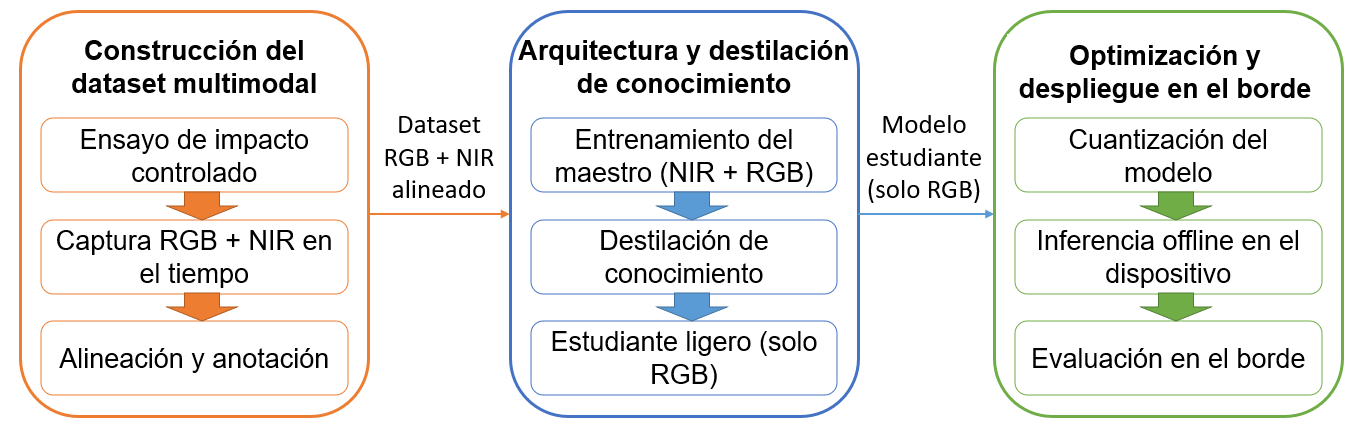
\includegraphics[width=0.7\textwidth]{fig2_workflow.png}
\caption{Complete methodological workflow.}
\label{fig:workflow}
\end{figure*}

\subsection{Methodological Workflow}\label{sec:workflow}
\textbf{Multimodal dataset construction.} Each fruit is photographed in RGB and NIR before a standardized impact, identical for all samples, and then at fixed intervals during the following 12 hours. A 66~g steel sphere of about 25~mm in diameter falls freely, guided by a PVC tube, from 50~cm above the fruit, which rests on viscoelastic foam, applying a nominal energy of 0.32~J, following the free-falling sphere method to induce controlled bruises~\cite{pathare2021}. Since the two cameras are physically separated, both images are aligned through a homography (Fig.~\ref{fig:dataset-process}).

\begin{figure*}[!t]
\centering
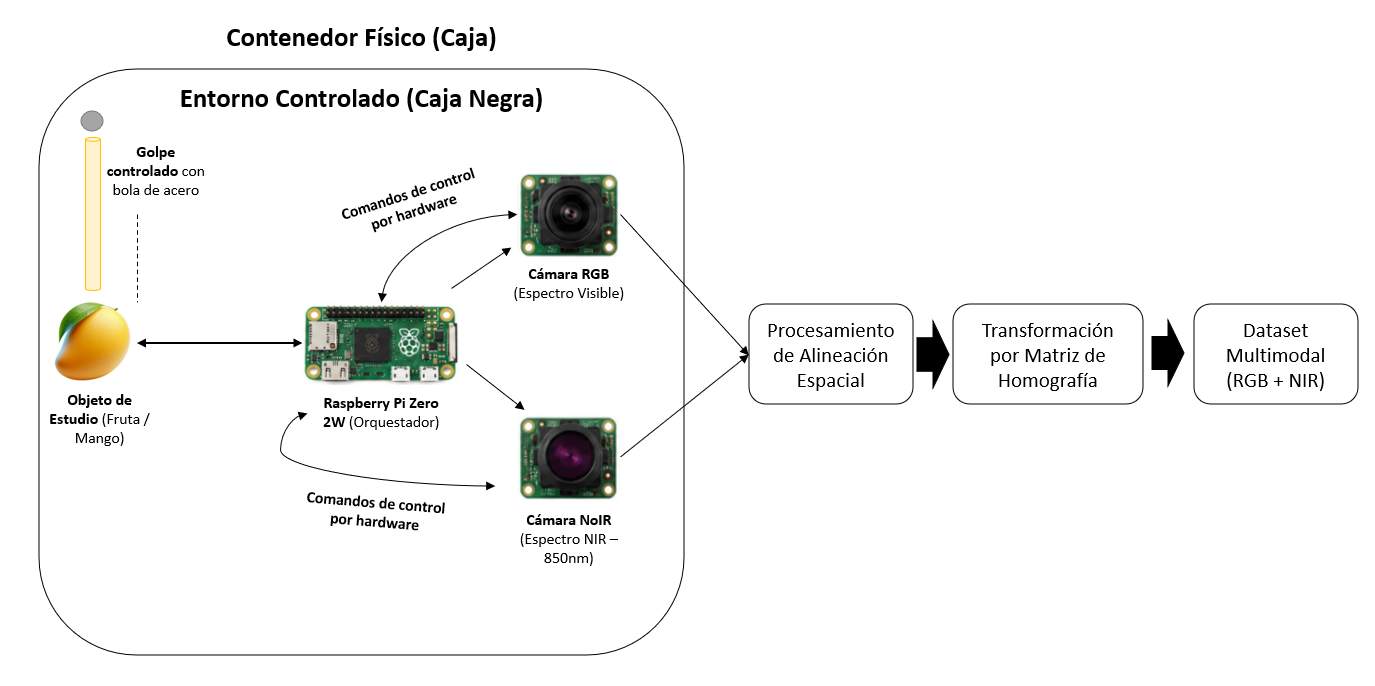
\includegraphics[width=0.65\textwidth]{fig3_dataset_process.png}
\caption{Methodological process for dataset creation.}
\label{fig:dataset-process}
\end{figure*}

The capture is performed in a closed box with constant illumination, distance and fruit position, so that the differences between images respond mainly to the spectral information of the fruit. A Raspberry Pi Zero 2W sequentially coordinates an RGB camera, equivalent to a commercial sensor, and a NoIR camera at 850 nm. After aligning the NIR image onto the RGB plane, each sample is a registered pair of a three-channel RGB image and a one-channel NIR image; the model that uses both modalities receives them stacked in a four-channel tensor from the first layer.

Before training the models, a patch-wise logistic regression measures, at each hour and modality, whether the impacted zone can be distinguished from a control zone, leaving one lot out in each iteration. This analysis estimates how much signal each modality contains without depending on a deep network.

\textbf{Architecture and knowledge distillation.} This phase employs two models with the same YOLOv8n-seg architecture, which predicts the box and the mask of each instance. The teacher receives the RGB and the NIR image stacked in four channels (early fusion) and is trained only with the labels; its first convolution is adapted to the four channels, so that the only difference from the student is the input information. The student processes only RGB images, because that is the information available in a packing plant, and is trained with the labels and with the CrossKD distillation loss of Eq.~\eqref{eq:loss} (Fig.~\ref{fig:kd}).

\begin{figure*}[!t]
\centering
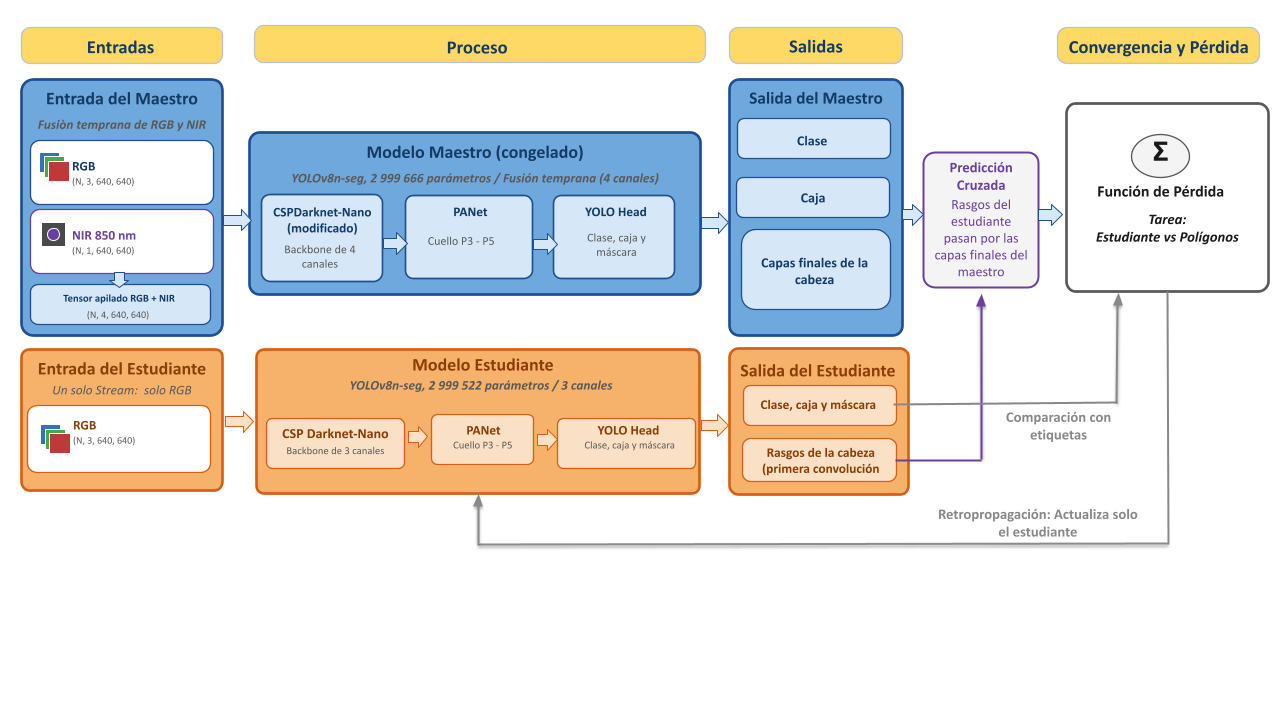
\includegraphics[width=0.7\textwidth]{fig4_kd_training.png}
\caption{Multimodal training process (knowledge distillation).}
\label{fig:kd}
\end{figure*}

During distillation, the teacher remains frozen. At each level of the head, the student's intermediate features pass through the remaining layers of the teacher's head, and the class and box thus obtained are brought closer to the teacher's own predictions. Backpropagation updates only the student, which is penalized for the differences that change the teacher's detection decision and not for failing to reproduce features that exist only in the NIR. Distillation acts on the class and the box; the mask is learned only from the labels, because the mask prototypes of two networks are not comparable with each other.

To evaluate the contribution of the NIR and of distillation, an ablation study is performed with five configurations of the same architecture, which differ only in the input or in the distillation teacher (Table~\ref{tab:arms}). All are trained and evaluated on the same five folds, so that each comparison is a lot-paired design.

\begin{table}[!t]
\caption{Experimental arms}
\label{tab:arms}
\centering
\scriptsize
\setlength{\tabcolsep}{3pt}
\renewcommand{\arraystretch}{1.1}
\begin{tabular}{@{}p{1.8cm}p{1.0cm}p{1.9cm}p{3.1cm}@{}}
\toprule
Arm & Input & Training & Role \\
\midrule
\texttt{master\_\allowbreak rgb} & RGB & Labels only & Baseline of H1 and teacher of \texttt{crosskd\_\allowbreak rgb} \\
\texttt{master\_\allowbreak rgbnir} & RGB + NIR & Labels only & Treatment of H1 and teacher of \texttt{crosskd\_\allowbreak rgbnir} \\
\texttt{crosskd\_\allowbreak rgb} & RGB & CrossKD from \texttt{master\_\allowbreak rgb} & Baseline of H2 \\
\texttt{crosskd\_\allowbreak rgbnir} & RGB & CrossKD from \texttt{master\_\allowbreak rgbnir} & Treatment of H2 \\
\texttt{master\_\allowbreak nir} & NIR & Labels only & Descriptive reference \\
\bottomrule
\end{tabular}
\end{table}

With these arms, two hypotheses and two additional comparisons are contrasted (Table~\ref{tab:hyp}).

\begin{table*}[!t]
\caption{Hypotheses and comparisons of the experiment}
\label{tab:hyp}
\centering
\footnotesize
\renewcommand{\arraystretch}{1.1}
\begin{tabular}{@{}lp{10cm}ll@{}}
\toprule
Comparison & Statement & Baseline & Treatment \\
\midrule
H1 & With the same architecture, adding the NIR image to the RGB at the input improves the detection of latent damage ($t \le 6$~h) & \texttt{master\_\allowbreak rgb} & \texttt{master\_\allowbreak rgbnir} \\
H2 & An RGB student distilled from an RGB + NIR teacher outperforms one distilled from an RGB teacher & \texttt{crosskd\_\allowbreak rgb} & \texttt{crosskd\_\allowbreak rgbnir} \\
C1 & An RGB student distilled from an RGB + NIR teacher outperforms the RGB teacher without distillation & \texttt{master\_\allowbreak rgb} & \texttt{crosskd\_\allowbreak rgbnir} \\
C2 & Distilling from a teacher of the same modality improves the RGB model & \texttt{master\_\allowbreak rgb} & \texttt{crosskd\_\allowbreak rgb} \\
\bottomrule
\end{tabular}
\end{table*}

H1 is tested first, and H2 is read as the main finding only if H1 is favorable. The control with an RGB teacher (\texttt{crosskd\_\allowbreak rgb}) is necessary because distillation can improve a student even when the teacher sees the same modality; without it, an improvement of \texttt{crosskd\_\allowbreak rgbnir} over \texttt{master\_\allowbreak rgb} could not be attributed to the NIR. In each fold, the checkpoint with the highest damage AP50 on validation is chosen, and that model is evaluated only once on the test lot.

\textbf{Optimization and edge deployment.} Finally, the distilled student is exported to LiteRT and runs offline on a phone, where the NIR camera no longer intervenes. FP32, FP16 and INT8 versions are evaluated, whose lower numerical precision reduces size and latency, and their latency, throughput, memory and size are measured (Fig.~\ref{fig:edge-process}).

\begin{figure*}[!t]
\centering
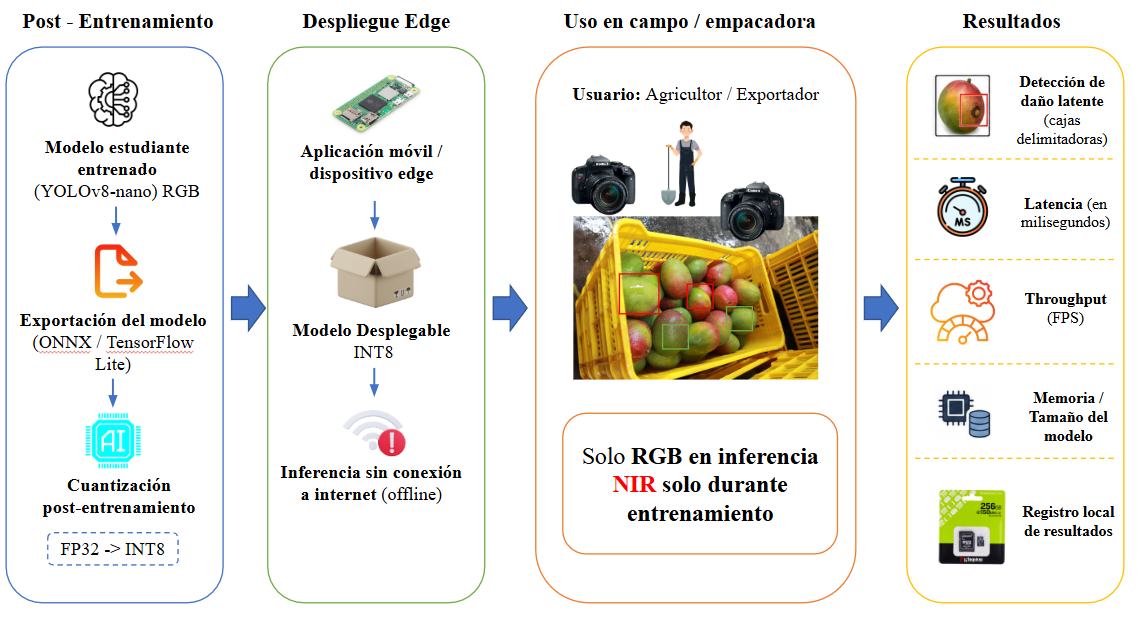
\includegraphics[width=0.65\textwidth]{fig5_edge_deploy.png}
\caption{Edge deployment process.}
\label{fig:edge-process}
\end{figure*}

The model trained in PyTorch is converted directly to LiteRT, without an intermediate ONNX representation, and integrated into an Android application that captures the image of the fruit, crops the mango and generates the predictions locally. Thus, the system requires only a commercial RGB camera, which facilitates its adoption by exporters and quality inspectors without specialized spectral hardware.

\section{Experimentation}\label{sec:exp}

\subsection{Experimental Setup}\label{sec:setup}
The experiment hardware is divided into three parts:
\begin{itemize}
\item \textbf{Capture:} a Raspberry Pi Zero 2W controls an Arducam IMX219 camera connected by USB for the RGB (3264 $\times$ 2448 px) and a Raspberry Pi NoIR v2 module without IR filter (3280 $\times$ 2464 px) for the NIR. The illumination alternates a white LED for the RGB shot and 850 nm emitters for the NIR one, switched by relays from the GPIO pins, and a custom Python program controls the lights, the cameras, the quality control, the metadata and the capture schedule.
\item \textbf{Training:} an NVIDIA RTX 6000 Ada with 48 GB of VRAM, with 48 CPU threads and 128 GB of RAM.
\item \textbf{Edge inference:} a Xiaomi 14T phone with a MediaTek Dimensity 8300-Ultra SoC, which includes a CPU, a GPU and a dedicated NPU.
\end{itemize}

The software consists of:
\begin{itemize}
\item \textbf{Training:} Python 3.12 and PyTorch 2 with CUDA. The task loss combines Focal Loss for classification~\cite{lin2017}, CIoU for box regression~\cite{zheng2020} and a per-pixel binary cross-entropy for the mask, with a task-aligned label assignment~\cite{feng2021}.
\item \textbf{Preprocessing:} OpenCV estimates the homography from ArUco markers and registers the NIR image onto the RGB plane.
\item \textbf{Export and deployment:} litert-torch converts the student to LiteRT, with a numerical parity test against the original model, and a Kotlin application with LiteRT 2.3.2 runs it on the phone.
\end{itemize}

\subsection{Data Description}\label{sec:data}
\subsubsection{Nature and structure of the dataset}\label{sec:structure}
The primary set consists of 125 Edwards mangoes, the unit of analysis, divided into five lots of 25, each captured in an independent session. 4000 RGB-NIR pairs are planned: 500 of healthy faces (125 mangoes $\times$ 4 faces, before the impact) and 3500 with damage (125 mangoes $\times$ 4 faces $\times$ 7 moments: immediately after the impact and then every 2 hours, up to 12 hours).

The pairs are grouped into three states: healthy, which acts as a negative of the same face; latent damage, from 0 to 6 hours after the impact; and developed damage, from 8 to 12 hours.

\subsubsection{Geometric correction (homography)}\label{sec:homography}
Given the physical parallax between the RGB sensor and the NIR sensor of the stereoscopic arrangement, a two-step spatial alignment preprocessing is applied. First, in each session a static homography is calibrated with a board of ArUco markers~\cite{garrido2014} (dictionary DICT\_4X4\_50), placed at the height of the top of the fruit. Using the OpenCV library, the markers are detected in both images, matched by identifier, and the two-dimensional homography matrix relating the RGB plane to the NIR plane is estimated with RANSAC~\cite{fischler1981}. Its inverse projects the NIR image onto the RGB plane. The matrix is calibrated in each session because it is not transferable between sessions, since any displacement of the camera support invalidates it.

Since the fruit protrudes from the plane of the board, the homography leaves a residual displacement over the fruit. Therefore, an additional translation is applied to each photo, the one that maximizes the correlation between the gradients of the RGB image and those of the registered NIR within the fruit mask. Fig.~\ref{fig:aruco} shows the board used to estimate the homography.

\begin{figure}[!t]
\centering
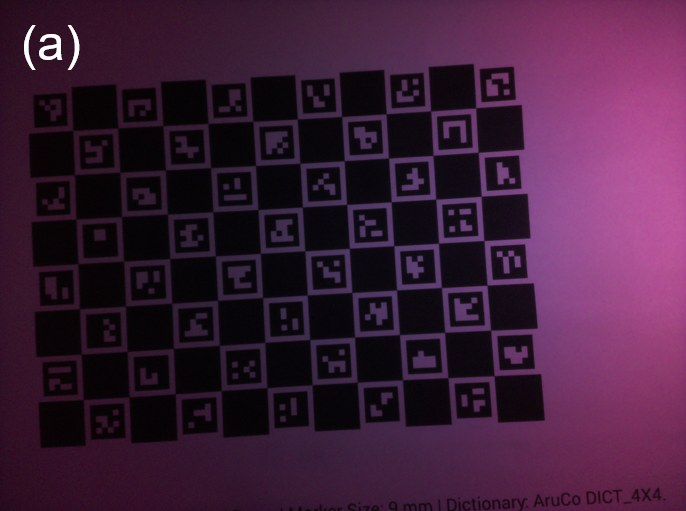
\includegraphics[width=0.48\columnwidth]{fig6a_aruco_nir.jpg}\hfill
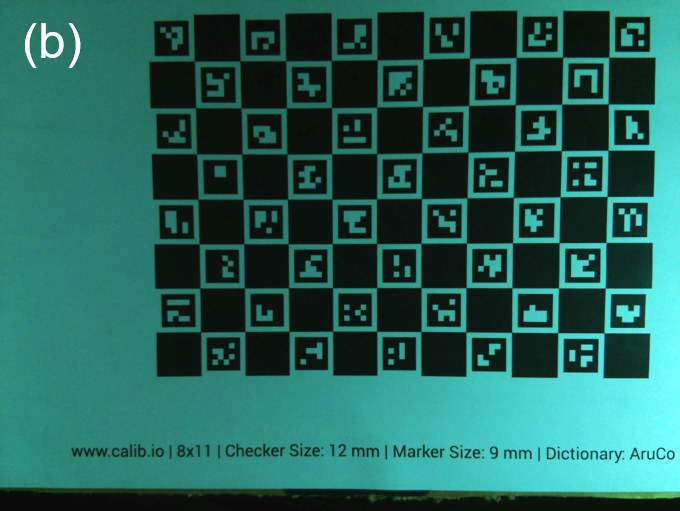
\includegraphics[width=0.48\columnwidth]{fig6b_aruco_rgb.jpg}
\caption{ArUco board for the homography matrix. (a) Capture from the NIR camera. (b) Capture from the RGB camera.}
\label{fig:aruco}
\end{figure}

\subsubsection{Polygon annotation}\label{sec:annotation}
The fruit and the damage are annotated with different strategies (Fig.~\ref{fig:annotation}):
\begin{itemize}
\item \textbf{Class 0 (mango):} the contour of the fruit is obtained automatically from a color mask, which separates the mango pixels from the cyan background of the capture box in the CIELAB space.
\item \textbf{Class 1 (damage):} the bruise is delimited manually with a polygon in Label Studio, with the RGB and the NIR image of the same shot side by side; since the NIR is already registered onto the RGB, the polygon falls directly on the training plane. One polygon is drawn per photo, on the modality in which the damage is best seen: the CLAHE-enhanced NIR in the latent window and, more frequently, the RGB when the damage is already developed; whether the damage is visible in RGB and in NIR is also recorded. The polygons replaced a first annotation with boxes, because a rectangular box includes healthy skin around a rounded lesion. The box of each damage, which is used by the primary metric, is derived from the polygon.
\end{itemize}

\begin{figure}[!t]
\centering
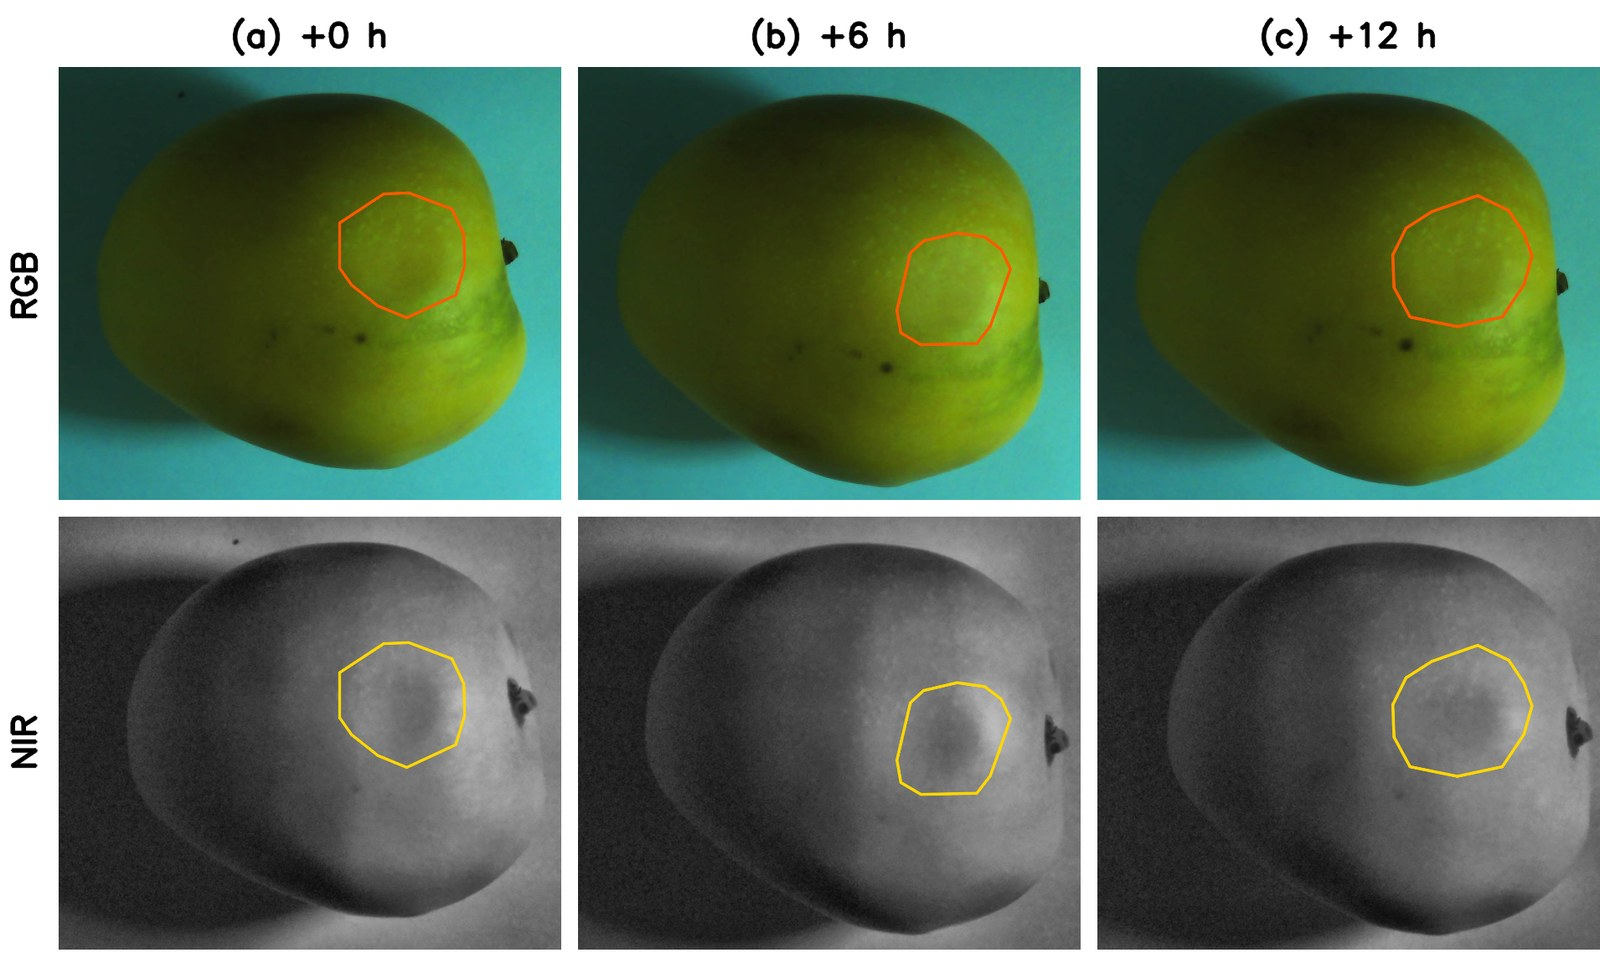
\includegraphics[width=\columnwidth]{fig7_annotation.jpg}
\caption{Damage annotation with polygons on the RGB and NIR images at (a) 0~h, (b) 6~h and (c) 12~h after the impact (lot 3, mango 62, face 1).}
\label{fig:annotation}
\end{figure}

\subsubsection{Partition strategy and online augmentation}\label{sec:partition}
The partition is performed by lot, with a five-iteration leave-one-lot-out cross-validation: in fold $k$ (from 0 to 4), lot $k+1$ is reserved for testing, the next lot for validation and the remaining three (75 mangoes) for training. Thus, the 32 shots of each fruit always remain in the same partition and, since each lot is a session with its own white balance and its own homography, the scheme measures the generalization to an unseen session. The NIR normalization statistics are computed only with the training set of each iteration, and the imbalance of the damage class is compensated with class weights (0.5 for mango and 1.5 for damage).

Since the mango occupies a small fraction of the frame, each pair is cropped around the mango box with a margin of 10\% per side and rescaled to 640 $\times$ 640 px; during training, the margin varies randomly. The evaluation therefore measures the detection of damage within an already localized fruit. The NIR image is enhanced with CLAHE before being normalized.

During training, an online augmentation is applied with Albumentations~\cite{buslaev2020}. The geometric transformations (flips, rotations and a slight perspective) are applied equally to the RGB image, the NIR image and the polygons, and the photometric ones (brightness, contrast, hue, blur, noise and patch occlusion) are applied only to the RGB, to preserve the reflectance measured in the NIR.

\subsection{Procedure}\label{sec:procedure}
\subsubsection{Data collection}\label{sec:collection}
The capture protocol was identical in the five lots, each in a continuous session of about 14 hours. Each session began with a calibration: a gray card fixed the white balance of the RGB camera, the empty tray served as a brightness reference and an ArUco board allowed estimating the homography of that session.

Then the four faces of each healthy mango were photographed, with an RGB shot under white light and a NIR one under 850 nm emitters. Each face received an impact at a zone randomly drawn among five positions and was captured immediately ($t = 0$~h) and in six more rounds, from +2 to +12~h, with a tolerance of 10 minutes with respect to the impact time of each fruit. Shots outside the tolerance were excluded, except for two exceptions defined before training, which remain within the window of their round: the +4~h round of lot 4 (100 shots, with a delay of 19 to 32 min) and that of three mangoes of lot 5 (12 shots, with a delay of 12 to 14 min).

An automatic quality control compared each shot with the brightness reference and rejected, to be repeated, those that differed by more than 30\%. Each pair keeps its metadata of lot, mango, face, moment, impact zone and actual elapsed hours. Fig.~\ref{fig:capture} shows the capture environment.

\begin{figure}[!t]
\centering
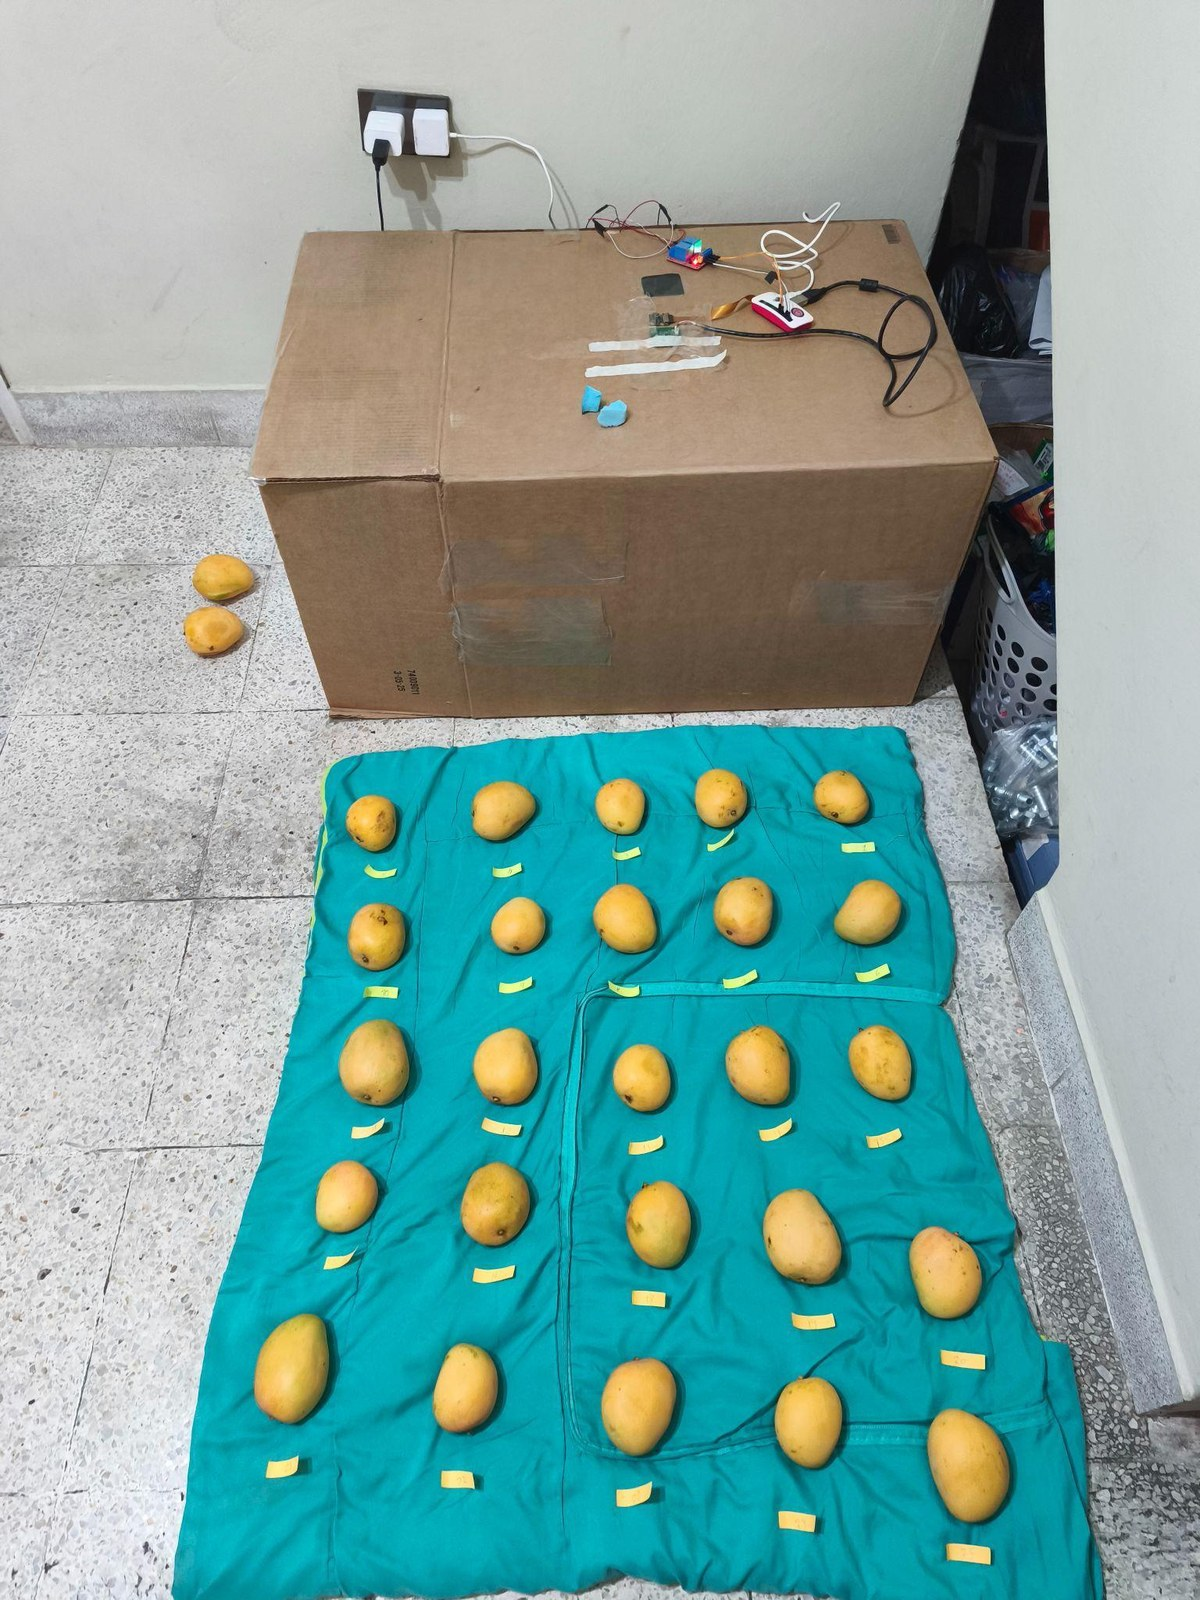
\includegraphics[width=0.6\columnwidth]{fig8_capture.jpg}
\caption{Capture environment.}
\label{fig:capture}
\end{figure}

\subsubsection{Modeling and distillation}\label{sec:modeling}
All arms start from the same YOLOv8n-seg architecture, initialized with COCO-pretrained weights, and share the hyperparameters of Table~\ref{tab:hyper}. They were optimized with AdamW~\cite{loshchilov2019}, with a learning rate of 0.001, a linear warm-up of three epochs and a cosine decay up to epoch 80, without early stopping, so that all received the same number of updates.

\begin{table}[!t]
\caption{Hyperparameters common to all arms}
\label{tab:hyper}
\centering
\scriptsize
\setlength{\tabcolsep}{3pt}
\renewcommand{\arraystretch}{1.1}
\begin{tabular}{@{}p{2.8cm}p{5.3cm}@{}}
\toprule
Parameter & Value \\
\midrule
Initialization & YOLOv8n-seg pretrained on COCO \\
Input size & 640 $\times$ 640 px, mango crop with 10\% margin \\
Epochs & 80, no early stopping \\
Optimizer & AdamW, learning rate 0.001, weight decay 0.0005 \\
Batch size & 8 \\
Loss weights & 7.5 for box and mask, 0.5 for class \\
Class weights & 0.5 for mango and 1.5 for damage \\
Checkpoint selection & Highest damage AP50 on validation \\
Distillation (\texttt{crosskd\_\allowbreak rgb} and \texttt{crosskd\_\allowbreak rgbnir}) & CrossKD, $\lambda_{\mathrm{cls}} = \lambda_{\mathrm{reg}} = 1.0$ \\
Seed & 42 \\
Student parameters & 3,354,818 \\
\bottomrule
\end{tabular}
\end{table}

Training was done in two phases within each fold. First the three teachers were trained with the labels only; then \texttt{master\_\allowbreak rgb} and \texttt{master\_\allowbreak rgbnir} were loaded frozen as the teachers of \texttt{crosskd\_\allowbreak rgb} and \texttt{crosskd\_\allowbreak rgbnir} in the same fold, so that each student learned from a teacher that never saw its test lot. Apart from the distillation loss, the students used the same hyperparameters as the teachers.

\subsubsection{Edge deployment}\label{sec:deployment}
The \texttt{crosskd\_\allowbreak rgbnir} student of fold 0, chosen for its latent AP50 on validation, was exported from PyTorch to LiteRT with litert-torch, without an intermediate ONNX representation. The model receives a 640 $\times$ 640 px RGB image and returns the undecoded boxes, the class logits, the mask coefficients and the prototypes; the decoding, the non-maximum suppression and the assembly of the masks are executed in the application. In addition to the FP32 version, FP16 and INT8 versions were generated, and each was evaluated on the validation set of the same fold.

The Android application was developed in Kotlin with CameraX and LiteRT 2.3.2, and allows choosing between the CPU, the GPU and the NPU of the phone. It operates in two modes. In the color-crop mode, it crops the mango with the same segmentation and the same 10\% margin used in training (Fig.~\ref{fig:app}). In the two-stage mode, intended for uncontrolled backgrounds, a YOLO11n detector pretrained on COCO and without fine-tuning first localizes the fruits in the full frame, and its apple, orange or banana detections are accepted as mango; the damage detector is then run on the crop of each fruit. It was chosen because two mango detectors trained for this work, with synthetic images and with public photographs, found the mango in only 6 of 17 public photographs of the whole fruit, against 15 of 17 for the exported YOLO11n. An IoU-based tracker assigns each fruit a stable identifier and keeps it for up to five frames if the detector loses it.

\begin{figure}[!t]
\centering
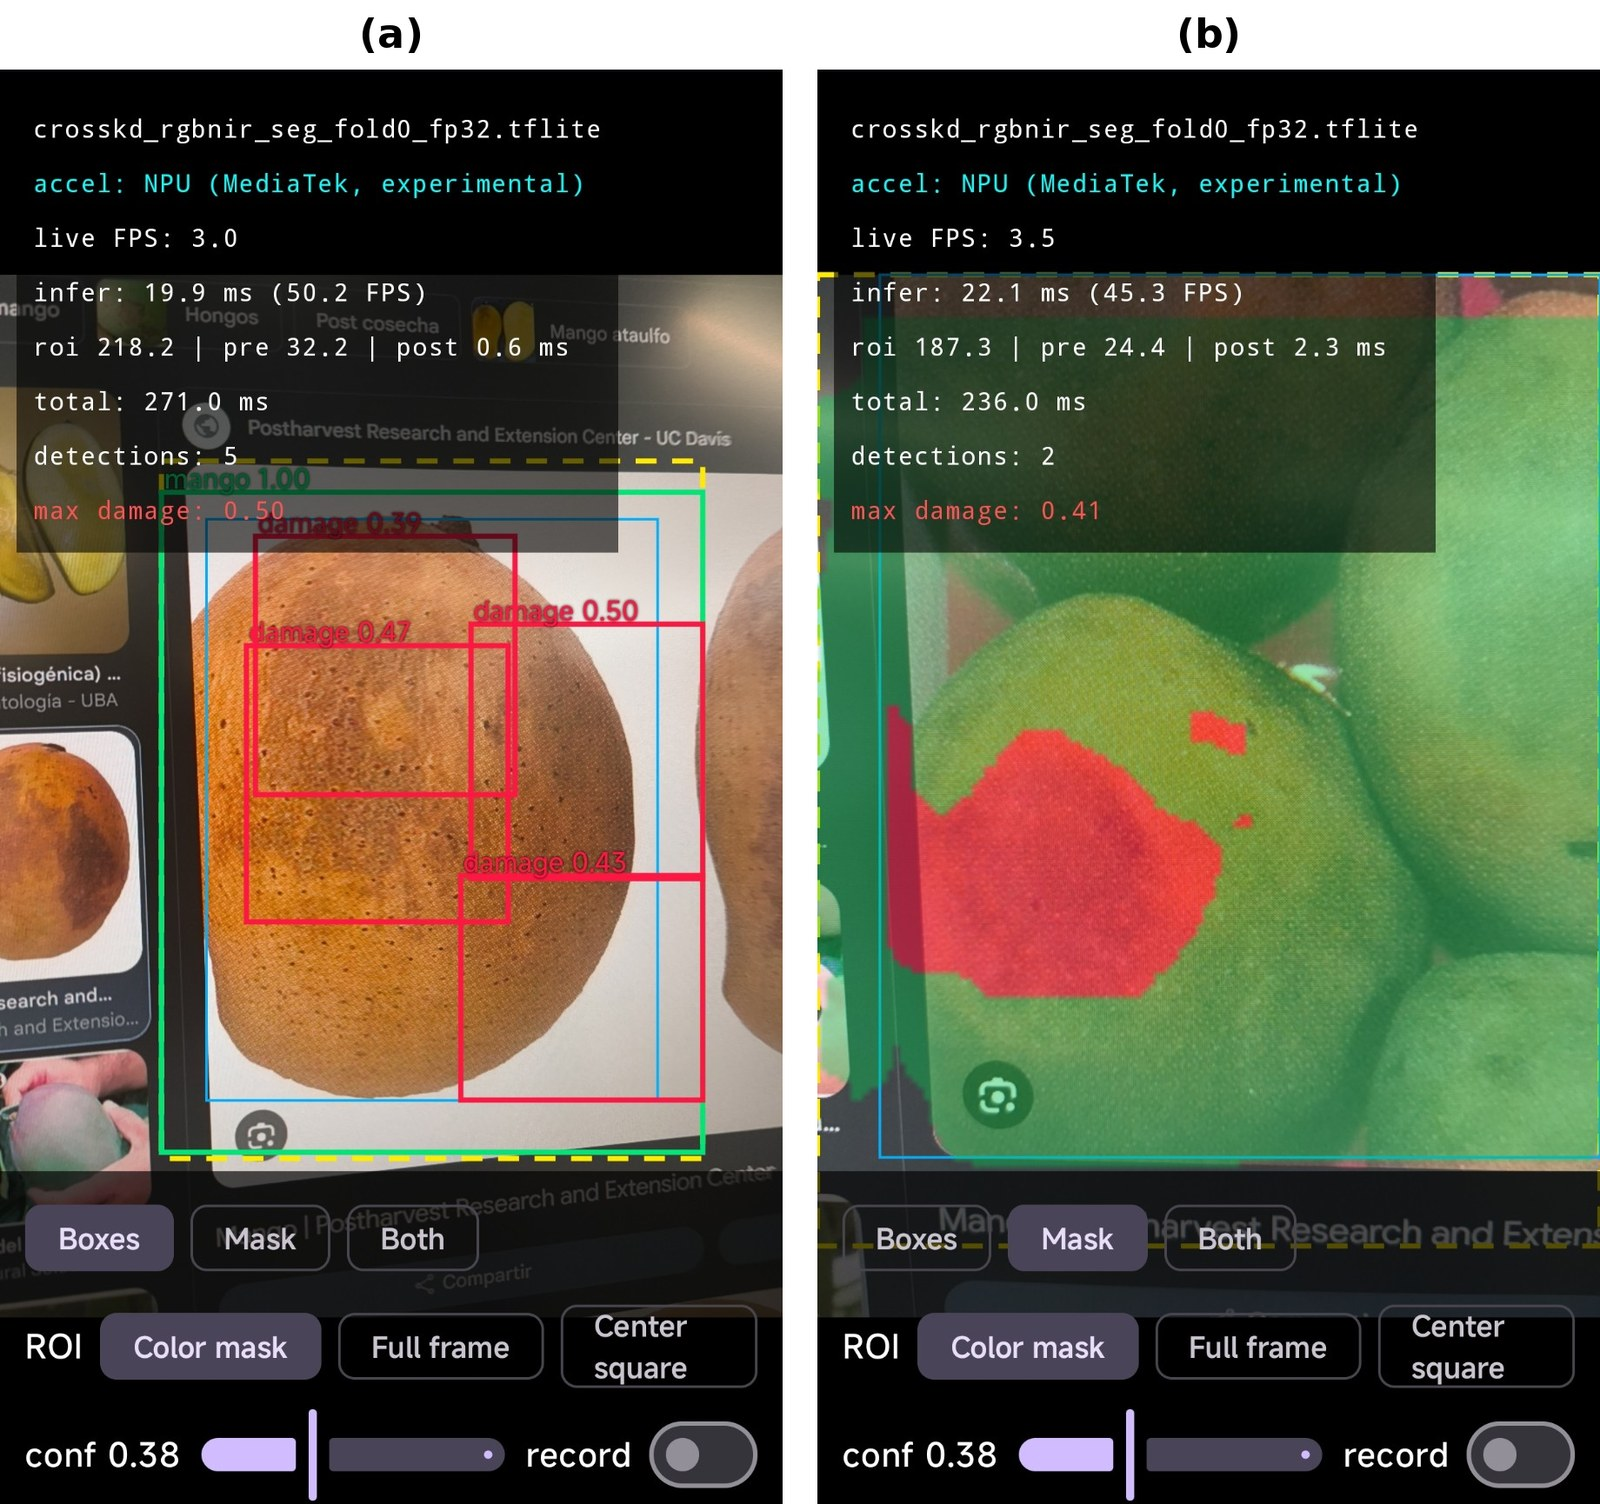
\includegraphics[width=\columnwidth]{fig9_app.jpg}
\caption{Edge-Mango application running the \texttt{crosskd\_rgbnir} student on the NPU of the Xiaomi 14T: (a) detection with boxes and (b) damage mask.}
\label{fig:app}
\end{figure}

In (a), the model localizes the mango (green box) and candidate damage regions (red boxes); in (b), the damage mask (red) is overlaid on the fruit. Both images are photographs shown on a screen, so they illustrate the application and do not constitute an evaluation.

In the two-stage mode, each session stores the analyzed frames, the boxes, masks and confidences of both detectors, the times of each stage and the memory of the process (RSS, process peak and PSS). Performance was measured with the six combinations of accelerator and precision of the damage detector, pointing the phone at the same image of a pile of mangoes shown on a screen. In addition, on November 22, 2026, the phone was passed over the piles of mangoes at a market stall, without handling the fruits, in sessions of 15 to 30 s. The detections were analyzed with the operating threshold of 0.25. Since the history of the fruits was not known and the damage was not annotated, the market test describes the behavior of the system and not its accuracy.

\subsection{Performance Metrics}\label{sec:metrics}
The primary metric is the box AP50 of the damage class in the latent window: a prediction is a hit if the IoU of its box with the box derived from the annotated polygon is at least 0.5. It is computed over the latent and healthy photos of the test lot. The mAP is not used, because the mango class saturates (AP50 of 1.0 in all arms) and hides the performance on damage.

As secondary metrics, the box AP30, the mask AP50, the per-face AUROC, with healthy photos as negatives and latent ones as positives, and the false positives per healthy photo with a confidence threshold of 0.25 are measured.

Each hypothesis is analyzed with the paired differences of the five folds. The confidence interval is corrected for the overlap between the training sets of the folds~\cite{nadeau2003}, and a Bayesian analysis estimates the probability that the difference falls above, within or below a region of practical equivalence (ROPE) of $\pm 0.02$ AP50~\cite{benavoli2017}. A comparison is favorable when the probability of exceeding that region is at least 0.95. These criteria were fixed before reading the test results.

The operating performance is measured on the Xiaomi 14T with 10 warm-up runs and 100 timed runs per configuration: latency per image (ms), FPS, peak memory (MB) and model size, together with their parameters and FLOPs.

\section{Results}\label{sec:results}
\subsection{Construction of the Multimodal Dataset}\label{sec:res-dataset}
The five sessions were carried out between October 24 and November 1, 2026, with an ambient temperature of 24.5 to 26 $^\circ$C and the RGB exposure and white balance fixed within each session (4600 to 5300 K). Of the 4000 planned shots, 3997 were recorded and 31 were excluded: 28 for falling outside the time tolerance, one face whose identity could not be confirmed, one shot whose NIR image did not contain the fruit and one without damage annotation. The final dataset contains 3966 RGB-NIR pairs, 99.2\% of what was planned (Table~\ref{tab:dataset}).

\begin{table}[!t]
\caption{Dataset composition by lot and damage state}
\label{tab:dataset}
\centering
\scriptsize
\setlength{\tabcolsep}{3pt}
\renewcommand{\arraystretch}{1.1}
\begin{tabular}{@{}cccccrr@{}}
\toprule
Lot & Healthy & \begin{tabular}[c]{@{}c@{}}Latent\\(0--6 h)\end{tabular} & \begin{tabular}[c]{@{}c@{}}Developed\\(8--12 h)\end{tabular} & Total & Excluded & \begin{tabular}[c]{@{}r@{}}Not\\captured\end{tabular} \\
\midrule
1 & 100 & 399 & 292 & 791 & 9 & 0 \\
2 & 100 & 394 & 298 & 792 & 7 & 1 \\
3 & 100 & 397 & 300 & 797 & 3 & 0 \\
4 & 100 & 400 & 299 & 799 & 1 & 0 \\
5 & 100 & 397 & 290 & 787 & 11 & 2 \\
\midrule
Total & 500 & 1987 & 1479 & 3966 & 31 & 3 \\
\bottomrule
\end{tabular}
\end{table}

The homography of each session had a median error of 1.8 to 2.7 px at the board corners (p95 of 4.6 to 7.0 px, on images 3264 px wide; Table~\ref{tab:homography}) and was not transferable between sessions: that of lot 1, applied to the board of lot 2, fails by 32 px. In lot 3 two matrices were calibrated, because the cameras were reoriented after a restart during the +6~h round. The per-photo residual translation had a median magnitude of 10 to 177 px depending on the lot, and with it the gradient correlation between both modalities went from values of 0.04 to 0.45 to a median of 0.6 in all lots and moments.

\begin{table}[!t]
\caption{Homography error per session and residual correction over the fruit}
\label{tab:homography}
\centering
\scriptsize
\setlength{\tabcolsep}{3pt}
\renewcommand{\arraystretch}{1.1}
\begin{tabular}{@{}lcc@{}}
\toprule
Lot & \begin{tabular}[c]{@{}c@{}}Board error, median / p95 / max (px)\end{tabular} & \begin{tabular}[c]{@{}c@{}}Median residual\\translation (px)\end{tabular} \\
\midrule
1 & 2.0 / 6.0 / 7.8 & 10 \\
2 & 2.7 / 6.2 / 20.7 & 35 \\
3 (morning) & 1.8 / 7.0 / 9.5 & 120 \\
3 (afternoon) & 2.3 / 5.3 / 7.2 & 120 \\
4 & 2.0 / 4.6 / 11.9 & 152 \\
5 & 2.0 / 6.5 / 9.6 & 177 \\
\bottomrule
\end{tabular}
\end{table}

As capture artifacts, 48 NIR images (1.2\%) showed 1 px sensor lines; the 12 that crossed the fruit were interpolated. In addition, 57 RGB photographs of lot 1 in the +4~h round received a post-capture white balance correction.

Each of the 3466 post-impact photos has a damage polygon, and the 500 healthy photos have no annotated damage. The median damage polygon has 15 vertices and occupies 11.7\% of the area of the mango contour (interquartile range of 9.6 to 14.1\%). The 500 impacted faces were distributed among the five randomly drawn zones: center 111, right 102, left 99, top 99 and bottom 89. As seen in Fig.~\ref{fig:annotation}, in the latent photos the mark of the blow is barely hinted at in the RGB shot, while in the NIR it appears as a dark zone from the capture immediately after the impact.

In the latent window, 97.9\% of the polygons were drawn on the NIR image, and the annotator judged the damage visible in the NIR in 98.8\% of the photos and in the RGB in only 10.6\% (doubtful in 79.6\%). With developed damage, 73.4\% of the polygons were drawn on the RGB and the visibility in RGB rose to 73.6\%, against 95.7\% in the NIR. This judgment is subjective and was issued by a single person, so it describes the annotation and does not measure the signal.

In each iteration, the test set contains 25 mangoes and 787 to 799 photos (100 of them healthy), and the training set, 75 mangoes and 2370 to 2383 photos; no mango or session appears in more than one partition.

\subsection{Experimental Results}\label{sec:res-exp}
The patch-wise analysis showed a weak signal in both modalities. In the latent window, the mean per-fold AUROC between the impacted zone and the control zone was 0.58 to 0.60 with RGB, 0.55 to 0.62 with NIR and 0.57 to 0.62 with both; at 10 and 12 hours it rose to 0.64 with RGB and 0.65 with NIR, while the negative control remained between 0.49 and 0.53 in the latent hours. With local intensity statistics, the NIR showed no clear advantage over the RGB in the latent hours.

With the trained detectors, the difference between modalities does appear (Table~\ref{tab:ap50}). The RGB + NIR teacher outperformed the RGB teacher in all five lots, with a mean latent AP50 of 0.388 against 0.306, and the teacher that receives only NIR obtained the highest value (0.434). The two distilled students fell between the RGB and RGB + NIR teachers, with 0.354 for \texttt{crosskd\_\allowbreak rgbnir} and 0.318 for \texttt{crosskd\_\allowbreak rgb}.

\begin{table*}[!t]
\caption{Latent box AP50 of the damage class on the test lot of each fold (seed 42)}
\label{tab:ap50}
\centering
\footnotesize
\setlength{\tabcolsep}{6pt}
\renewcommand{\arraystretch}{1.1}
\begin{tabular}{@{}lccccc@{}}
\toprule
Fold (test lot) & \texttt{master\_\allowbreak rgb} & \texttt{master\_\allowbreak rgbnir} & \texttt{crosskd\_\allowbreak rgb} & \texttt{crosskd\_\allowbreak rgbnir} & \texttt{master\_\allowbreak nir} \\
\midrule
0 (lot 1) & 0.239 & 0.315 & 0.303 & 0.336 & 0.353 \\
1 (lot 2) & 0.398 & 0.525 & 0.388 & 0.490 & 0.558 \\
2 (lot 3) & 0.327 & 0.356 & 0.353 & 0.400 & 0.448 \\
3 (lot 4) & 0.228 & 0.339 & 0.219 & 0.229 & 0.374 \\
4 (lot 5) & 0.340 & 0.405 & 0.325 & 0.316 & 0.439 \\
\midrule
Mean $\pm$ sd & 0.306 $\pm$ 0.072 & 0.388 $\pm$ 0.083 & 0.318 $\pm$ 0.063 & 0.354 $\pm$ 0.097 & 0.434 $\pm$ 0.080 \\
\bottomrule
\end{tabular}
\end{table*}

Fig.~\ref{fig:curves} shows the training evolution averaged over the five folds. In panel (a), the detection loss (box and class) decreases similarly in the five arms, with no signs of divergence, and the teachers that receive NIR end with the lowest loss. In panel (b), the damage AP50 on validation of the NIR and RGB + NIR teachers separates from the rest from the first epochs and stabilizes near 0.41, while the RGB teacher and the two students stay between 0.35 and 0.37, with overlapping dispersion bands between lots.

\begin{figure*}[!t]
\centering
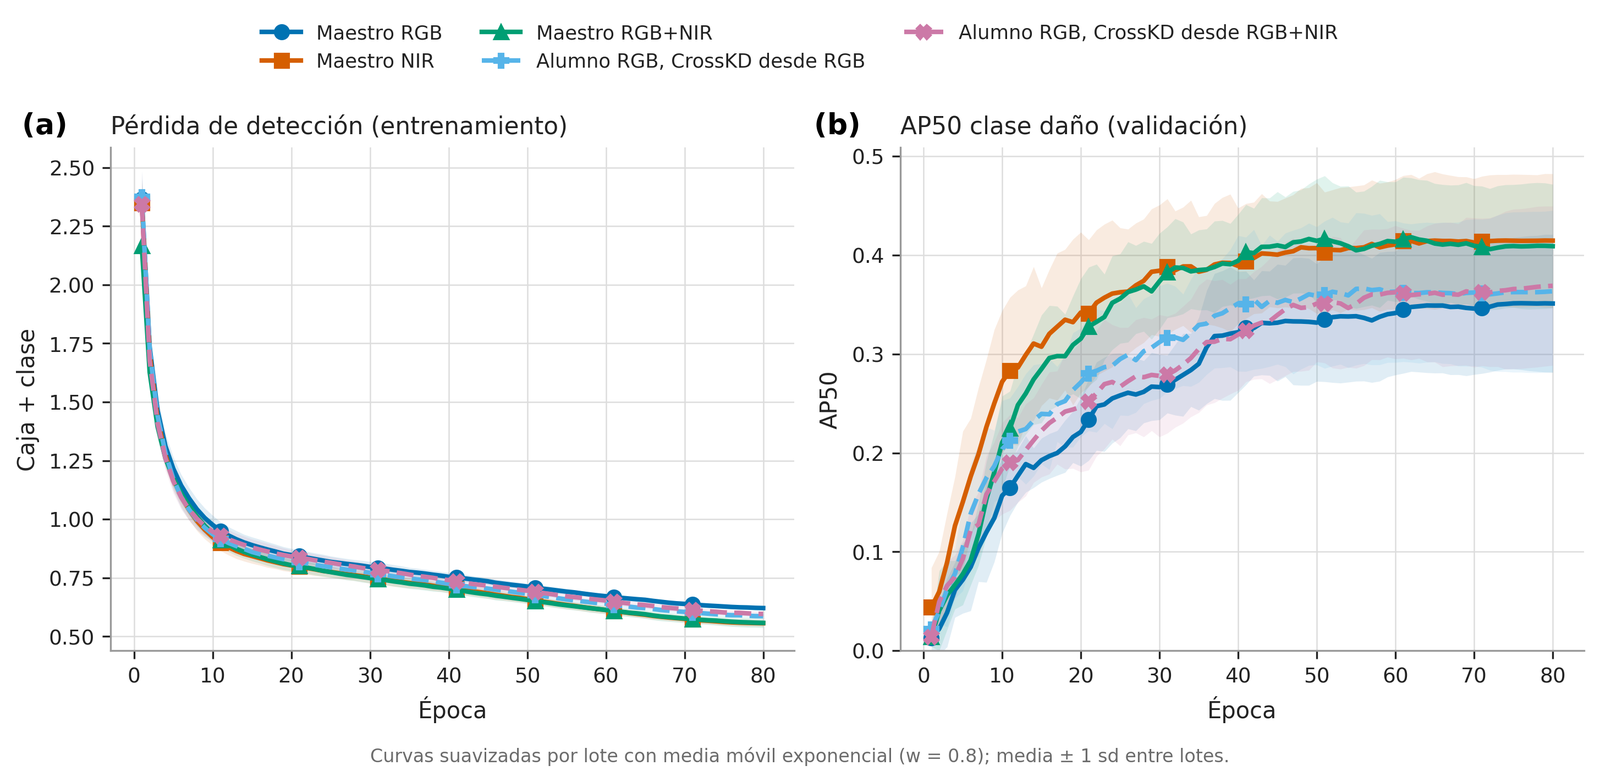
\includegraphics[width=0.8\textwidth]{fig10_curves.png}
\caption{Training curves averaged over the five folds (seed 42): (a) detection loss on training and (b) damage-class AP50 on validation.}
\label{fig:curves}
\end{figure*}

Table~\ref{tab:paired} and Fig.~\ref{fig:rope} present the paired analysis. In H1, the difference in favor of the NIR was +0.029 to +0.127 depending on the lot, with a mean of +0.082, four times the equivalence region; the corrected interval was +0.003 to +0.160 and the posterior probability of an improvement greater than 0.02 was 0.953, above the 0.95 threshold, so H1 is favorable according to the fixed criterion. In H2, the difference between the distilled students was +0.036, with four of five lots in favor of \texttt{crosskd\_\allowbreak rgbnir}, an interval of $-0.049$ to +0.122 and a probability of improvement of 0.689, so the result is inconclusive with five lots. Comparisons C1 and C2 were also inconclusive; in particular, the student distilled from the RGB teacher ended up practically equal to the RGB teacher (+0.011).

\begin{table}[!t]
\caption{Lot-paired analysis of the comparisons (latent box AP50, $n = 5$)}
\label{tab:paired}
\centering
\scriptsize
\setlength{\tabcolsep}{1.5pt}
\renewcommand{\arraystretch}{1.1}
\begin{tabular}{@{}lcccccc@{}}
\toprule
Comp. & Mean $\Delta$ & \begin{tabular}[c]{@{}c@{}}Corrected\\95\% CI\end{tabular} & P(worse) & \begin{tabular}[c]{@{}c@{}}P(equiv.)\end{tabular} & P(better) & \begin{tabular}[c]{@{}c@{}}Lots in\\favor\end{tabular} \\
\midrule
H1 & +0.082 & [+0.003, +0.160] & 0.011 & 0.036 & 0.953 & 5/5 \\
H2 & +0.036 & [$-$0.049, +0.122] & 0.071 & 0.240 & 0.689 & 4/5 \\
C1 & +0.048 & [$-$0.065, +0.160] & 0.085 & 0.181 & 0.734 & 4/5 \\
C2 & +0.011 & [$-$0.057, +0.080] & 0.137 & 0.493 & 0.371 & 2/5 \\
\bottomrule
\end{tabular}
\end{table}

\begin{figure*}[!t]
\centering
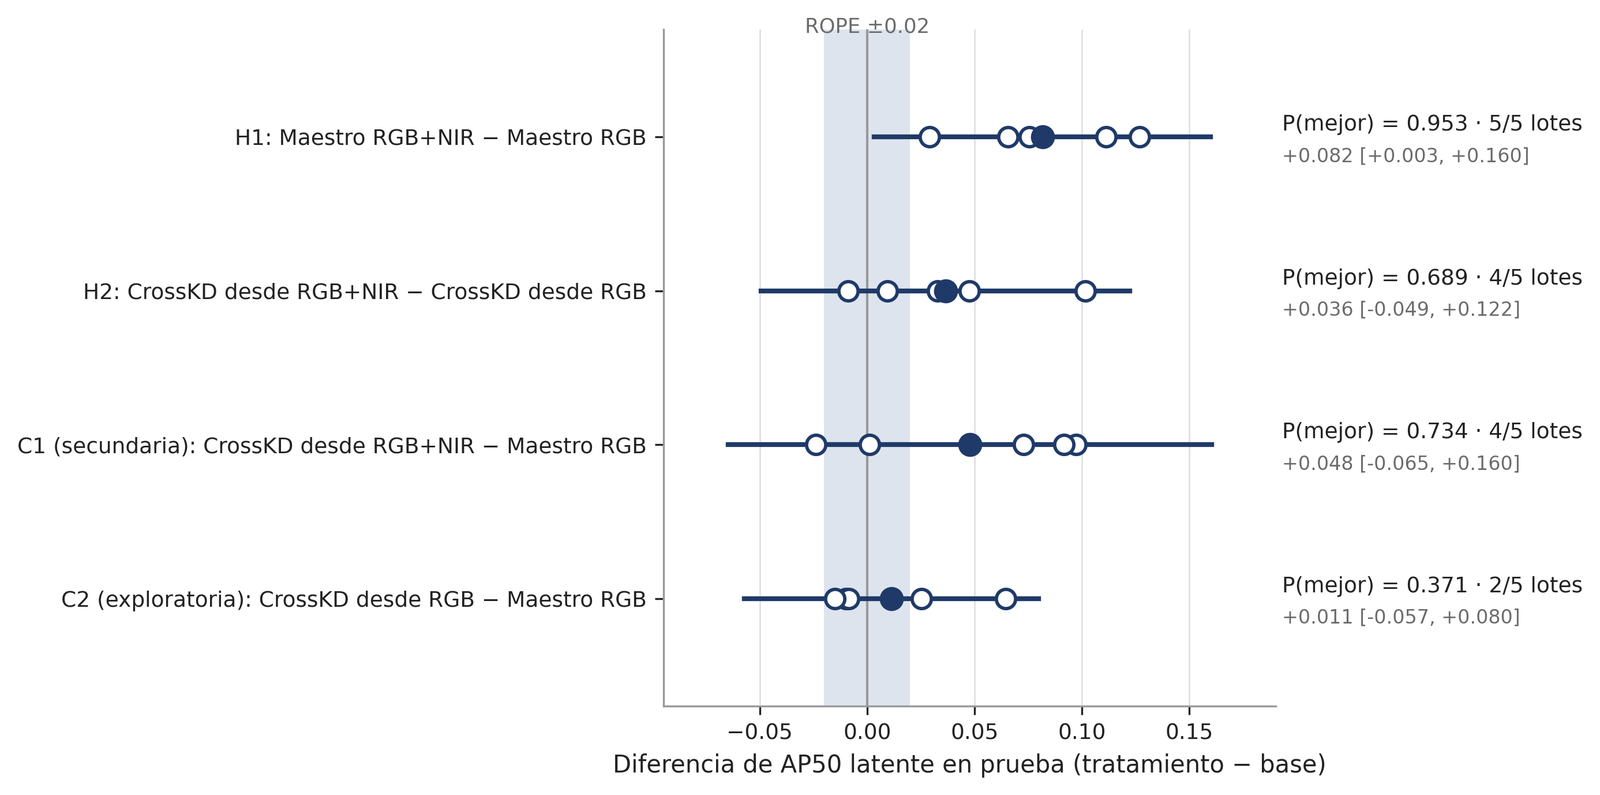
\includegraphics[width=0.7\textwidth]{fig11_rope.png}
\caption{Lot-paired differences against the region of practical equivalence (ROPE $\pm 0.02$) on test (seed 42).}
\label{fig:rope}
\end{figure*}

The secondary metrics follow the same order (Table~\ref{tab:secondary}). In H1, the advantage of the NIR was maintained in the AP30 (+0.091, with a probability of improvement of 0.980) and in the mask AP50 (+0.097, with a probability of 0.976), both with the five lots in favor. In contrast, the per-face AUROC stayed between 0.60 and 0.64 in the five arms, and all produced between 4.3 and 6.6 false detections per healthy photo with a threshold of 0.25, so deciding whether a face is damaged remains close to chance, even though the localization improves. As an exploratory analysis, a teacher with two separate stems for the RGB and the NIR, fused at intermediate levels, reached 0.377, without surpassing early fusion or the NIR teacher.

\begin{table}[!t]
\caption{Secondary metrics on test (mean of the five folds)}
\label{tab:secondary}
\centering
\scriptsize
\setlength{\tabcolsep}{3pt}
\renewcommand{\arraystretch}{1.1}
\begin{tabular}{@{}lcccc@{}}
\toprule
Arm & \begin{tabular}[c]{@{}c@{}}Latent\\AP30\end{tabular} & \begin{tabular}[c]{@{}c@{}}Mask\\AP50\end{tabular} & \begin{tabular}[c]{@{}c@{}}Per-face\\AUROC\end{tabular} & \begin{tabular}[c]{@{}c@{}}FP per\\healthy photo\end{tabular} \\
\midrule
\texttt{master\_\allowbreak rgb} & 0.445 & 0.295 & 0.599 & 5.76 \\
\texttt{master\_\allowbreak rgbnir} & 0.535 & 0.391 & 0.627 & 6.60 \\
\texttt{crosskd\_\allowbreak rgb} & 0.476 & 0.308 & 0.613 & 4.60 \\
\texttt{crosskd\_\allowbreak rgbnir} & 0.501 & 0.334 & 0.626 & 4.34 \\
\texttt{master\_\allowbreak nir} & 0.560 & 0.429 & 0.642 & 4.67 \\
\bottomrule
\end{tabular}
\end{table}

\subsection{Edge Deployment}\label{sec:res-edge}
The \texttt{crosskd\_\allowbreak rgbnir} student of fold 0 (latent AP50 on validation of 0.428; 3,354,818 parameters and 11.4 GFLOPs at 640 $\times$ 640 px) was measured only on the Xiaomi 14T. The NPU was the fastest accelerator, with 17.6 ms per image (56.8 FPS) in FP32, 2.4 times less than the GPU and 9.6 times less than the CPU; the FP16 version was rejected by the NPU. The INT8 version was the fastest and lightest, with 10.5 ms and 3.65 MB, but with the default quantization its latent AP50 on validation fell from 0.428 to 0.249, while the FP32 and FP16 versions kept the value of the original model.

The full two-stage system, with the YOLO11n mango detector (2,624,080 parameters, 6.6 GFLOPs and 5.4 MB in FP16), processed about five fruits per frame (Table~\ref{tab:system}). The NPU reached 1.25 frames per second with the damage detector in FP32 and was the configuration with the lowest memory, with a maximum RSS of 519 MB, against 612 to 645 MB with the GPU and 571 to 585 MB with the CPU. The mango detector in FP16 was not accelerated on the NPU and took 326 ms, against 67 ms on the GPU.

\begin{table*}[!t]
\caption{Performance of the two-stage system on the Xiaomi 14T (median per frame; mango detector in FP16)}
\label{tab:system}
\centering
\footnotesize
\setlength{\tabcolsep}{6pt}
\renewcommand{\arraystretch}{1.1}
\begin{tabular}{@{}llcccccc@{}}
\toprule
Accelerator & Damage & FPS & Total (ms) & Mango (ms) & Damage per fruit (ms) & Max RSS (MB) & Max PSS (MB) \\
\midrule
NPU & FP32 & 1.25 & 691 & 326 & 75 & 519 & 420 \\
NPU & INT8 & 1.14 & 816 & 329 & 80 & 519 & 419 \\
GPU & FP32 & 1.09 & 891 & 67 & 106 & 645 & 441 \\
GPU & INT8 & 1.23 & 833 & 69 & 128 & 612 & 514 \\
CPU & FP32 & 0.51 & 2060 & 172 & 275 & 585 & 429 \\
CPU & INT8 & 0.99 & 916 & 170 & 127 & 571 & 417 \\
\bottomrule
\end{tabular}
\end{table*}

In a real-environment test, the mango detector found at least one fruit in 71 to 100\% of the frames, with about 5 to 10 mangoes per frame on the piles and a median confidence of 0.37 to 0.58. The damage detector, in contrast, flagged damage with a confidence of at least 0.25 on all tracked fruits, with a median of 5 to 11 damage boxes per fruit. Without annotation its accuracy cannot be measured, but the damage detector did not discriminate between fruits.

\section{Discussion}\label{sec:discussion}
The clearest result of the study is that, with the same architecture and the same training, adding the NIR image to the input improves the localization of latent damage: the AP50 rose from 0.306 to 0.388, with the five lots in favor and a probability of 0.953 of exceeding the equivalence region, and the advantage was repeated in the AP30 and in the mask AP50. In addition, the teacher that receives only NIR obtained the highest value (0.434), which suggests that stacking the four channels at the input partly dilutes the infrared signal, although a teacher with two-stem intermediate fusion did not surpass it either (0.377). The margin is narrow, because the lower limit of the corrected interval is barely above zero (+0.003) and the difference does not withstand a post hoc correction for multiple comparisons; even so, the 850 nm image provides information about the lesion that the RGB does not contain to the same extent.

Distillation, in contrast, did not allow asserting that this advantage reaches the RGB student. The student guided by the RGB + NIR teacher outperformed the one guided by the RGB teacher in four of five lots (+0.036), but with a probability of improvement of 0.689 and an interval that includes zero. Furthermore, distilling from an RGB teacher did not improve on the model without distillation (+0.011), so the gain of \texttt{crosskd\_\allowbreak rgbnir} over the RGB teacher (+0.048) cannot be attributed with certainty to the NIR.

One possible explanation is that the student cannot reproduce what is not in its input. According to the modality focusing hypothesis of Xue \emph{et al.}~\cite{xue2023}, cross-modal distillation only transfers the decisive features that both modalities share, and what the teacher learns exclusively from its own does not help the student. In the latent window, the damage was judged visible in the RGB in only 10.6\% of the photos, against 98.8\% in the NIR, and the patch-wise analysis found no clear advantage of the NIR with local intensity statistics, so a good part of what the teacher learns from the NIR would have no counterpart in the RGB. In addition, the damage polygon occupies about 12\% of the area of the mango, so most of the cells that are compared do not contain a lesion. Yang \emph{et al.}~\cite{yang2022} showed that, in detection, concentrating the imitation on the regions of the objects prevents the background from dominating the distillation signal.

In comparison with the spectral works, V\'elez Rivera \emph{et al.}~\cite{velez2014} correctly classified 97.9\% of the damaged mango pixels on the third day with hyperspectral images, whereas in this study the RGB + NIR teacher reached an AP50 of 0.388 in the first six hours. Pourdarbani \emph{et al.}~\cite{pourdarbani2023} obtained 90.47\% accuracy when classifying lemons at 8 and 16 hours after the blow. Yao \emph{et al.}~\cite{yao2024} reached 93.48\% when estimating the time elapsed since the bruise in mango. Gulzar and \"Unal~\cite{gulzar2025} obtained 97.17\% when classifying healthy and bruised plums at 12 and 72 hours with NIR images. These values are higher, but they measure the classification of pixels or of fruits with hyperspectral cameras and partitions that share fruits, whereas here the localization of the lesion is measured with AP50 over sessions that the model did not see. They coincide, however, in direction: like Yuan \emph{et al.}~\cite{yuan2022}, who localized apple bruises in their first half hour with a 900 to 2350 nm NIR camera, here the NIR improved the localization from the capture immediately after the blow, with a commercial NoIR camera at 850 nm. Yan \emph{et al.}~\cite{yan2025} segmented pear bruises with an mIoU of 95.68\% also using a NIR camera, whereas here the RGB + NIR teacher reached a mask AP50 of 0.391; the difference reflects, besides the fruit, that here the detection over unseen sessions is evaluated and not the pixel overlap on a proprietary set. Compared with the 95.24\% accuracy of the thermal and spectral system of He \emph{et al.}~\cite{he2025}, the per-face AUROC of 0.60 to 0.64 indicates that, with this camera and this data volume, it is still not possible to reliably separate damaged faces from healthy ones. The same occurs against the 95.5\% that Y. Wang \emph{et al.}~\cite{wang2025} obtained with MECN-net.

In cross-modal distillation, Poojitha \emph{et al.}~\cite{poojitha2026} recovered 94\% of the mAP of an RGB-thermal teacher (75\% against 80\%) with an RGB student ten times smaller. In this study, the \texttt{crosskd\_\allowbreak rgbnir} student reached 91\% of the latent AP50 of the RGB + NIR teacher (0.354 against 0.388), but the RGB teacher without distillation already reached 79\%, so the gain attributable to distillation is smaller. J. Wang \emph{et al.}~\cite{wang2024} raised with CrossKD the AP of a detector on COCO from 40.2 to 43.7 (+3.5), whereas here distillation only showed a gain, inconclusive, with the RGB + NIR teacher (+0.048 AP50; probability of improvement of 0.734) and none with the RGB teacher (+0.011). The difference lies in the object being sought: in driving scenes, a good part of what the teacher sees in the thermal is also visible in the RGB, whereas the latent damage of the mango barely manifests in the visible. Huo \emph{et al.}~\cite{huo2024} identified that gap between modalities as the cause of the low performance of conventional distillation, and the results of this work are consistent with that explanation.

At the edge, the student ran in 17.6 ms per image on the phone's NPU (56.8 FPS in FP32), above the 28 FPS and 0.051 J per inference that Poojitha \emph{et al.}~\cite{poojitha2026} reported on an NVIDIA Jetson AGX Orin with TensorRT in FP16 and a student of 4.7 million parameters, against the 3.4 million of the present one; energy consumption was not measured in this work. The comparison changes when considering the full system: with a preceding mango detector and about five fruits per frame, the phone processed 1.25 frames per second with 519 MB of memory, because the damage detector is run once per fruit and the mango detector in FP16 was not accelerated on the NPU, whereas Poojitha \emph{et al.}~\cite{poojitha2026} evaluate a single model per image. Finally, the default INT8 quantization reduced the AP50 from 0.428 to 0.249 and, in the full system, did not accelerate the damage detector on the NPU (80 against 75 ms per fruit), so the version usable today is FP32.

The main limitation of the study is the number of lots: with five, each comparison rests on five differences, the intervals are wide by construction and the results correspond to a single seed, so the variability between seeds is not estimated. In addition, the annotation of latent damage was made mainly on the NIR image and by a single person, which may favor the models that receive the NIR. In the lot-wise evaluation, the fruit crop uses the mango contour also at test time; on the phone, that step is covered by an untuned COCO detector that treats any round fruit as mango. The captures were made with fixed light and camera and with a single impact level of 0.32 J, conditions necessary to control the variables, but different from a packing line. Finally, in the market the damage detector flagged all fruits, which evidences an important domain shift, from green Edwards mangoes on a cyan background to ripe mangoes in piles, and that test had neither ground truth nor energy measurements.

\section{Conclusions}\label{sec:conclusions}
This work built a set of 3966 aligned RGB-NIR pairs of 125 mangoes, with controlled impacts, seven captures over 12 hours and the damage annotated with polygons, and evaluated lot-wise whether the NIR helps to detect latent damage and whether distillation can bring that help to a segmenter that sees only RGB. With the same architecture, adding the NIR to the input raised the latent AP50 from 0.306 to 0.388, with improvements in the five lots and a probability of 0.953 of exceeding the equivalence region, above the fixed threshold, and the teacher that receives only NIR reached 0.434. Distillation with CrossKD, in contrast, gave an inconclusive result: the student guided by the teacher with NIR outperformed the one guided by the RGB teacher by +0.036, with a probability of 0.689.

The premise of the asymmetric approach, that the NIR contains useful information about latent damage, thus receives support, but it cannot be asserted that the chosen mechanism carries it over to the RGB, which is consistent with the idea that distillation only transfers what both modalities share. The student is viable on a commercial phone, with 17.6 ms per image on the NPU, and the full two-stage system ran offline at 1.25 frames per second with about five fruits per frame and 519 MB of memory; however, in a market the damage detector flagged all fruits, and the default INT8 quantization does not preserve accuracy. For the agro-industry, a commercial NoIR camera at 850 nm improves the localization of early damage, but with these data it still does not allow deciding reliably whether a face is damaged. Confirming these results requires more seeds, more lots and annotations independent of the NIR.

\section{Future Work}\label{sec:future}
In distillation, the next step is to center the imitation on the fruit and the damage, combine it with feature imitation and also distill the masks. In deployment, it is advisable to quantize with mixed calibration, run the mango detector in FP32 on the NPU, train one's own with market photos and adapt the damage one to ripe mangoes and uncontrolled scenes.

In capture, new sessions in other seasons and with diffuse light, instead of the fixed side light, would allow confirming the advantage of the NIR. In addition, a second person should annotate the damage on the RGB without seeing the NIR, to rule out a bias in favor of the models that receive it.

\section*{Declarations}
\subsection*{Ethics approval}
The manuscript will be evaluated by the Ethics Committee of the Universidad de Lima at a stage after this submission.

\subsection*{Consent to participate}
Not applicable (there is no direct dealing with human beings in the experiment).

\subsection*{Use of generative artificial intelligence}
During the preparation of the manuscript, the following were used: Gemini Pro 3.1 and Gemini Flash 3.8 for the correction of the writing and the review of inconsistencies. ChatGPT Work was used for the review and audit of the final document. In addition, Claude Code with Opus 5.5 was used for the design of the architecture and the implementation of the backpropagation and forward pass, as well as the training, preprocessing and inference pipelines. Cursor with Grok 4.7 was used, performing a functional validation of all the pipelines, generating tests for edge cases and automating the training runs. Finally, OpencodeGo was used with the models DeepSeek v4.1, GLM 5.1 and Kimi-K 3 for the first versions of the architectures.

\bibliographystyle{IEEEtran}
\bibliography{refs}

\end{document}
